% Joaquin Matres
%%%%%%%%%%%%%%%%%%%%%%% preamble %%%%%%%%%%%%%%%%%%%%%%%%%%%
\documentclass[10pt,letterpaper]{article}
\usepackage{opex3}
\usepackage{amsmath}

\usepackage{color}
\newcommand{\comment}[1]{\textcolor{red}{#1}}
\newcommand{\fWidthSetup}{0.85}
\newcommand{\fWidth}{0.8}

%\usepackage{ae} %%for Computer Modern fonts

%%%%%%%%%%%%%%%%%%%%%%% begin %%%%%%%%%%%%%%%%%%%%%%%%%%%%%%
\begin{document}

%%%%%%%%%%%%%%%%%% title page information %%%%%%%%%%%%%%%%%%
\title{Nonlinear Two-photon absorption loss measurement for pulsed lasers}
% Two-photon absorption nonlinear loss measurement with pulsed lasers
% Two-photon absorption nonlinear imaginary part measurement
%\title{Ultrafast nonlinear dynamics in silicon nanocrystal-based horizontal slot waveguides}

\author{J. Matres$^{*}$, G. C. Ballesteros, J. Mart\'i and C. J. Oton}
% J. Mart\'i$^1$,
\address{Nanophotonics Technology Center, \\ Universidad Polit\'ecnica de Valencia, Camino de Vera s/n, 46022, Valencia, Spain
}

\email{$^*$joamatab@ntc.upv.es}


%%%%%%%%%%%%%%%%%%% abstract and OCIS codes %%%%%%%%%%%%%%%%
%% [use \begin{abstract*}...\end{abstract*} if exempt from copyright]

\begin{abstract}
We present a correction of the commonly used method to determine the Two-photon absorption coefficient when using a pulsed laser and averaging power meters. Different equations are used to fit the imaginary part of the nonlinear coefficient depending on the shape of the pulses. With this method we compare the nonlinear losses of TE and TM Silicon strip waveguides.
\end{abstract}

% We review the measurement of the the Two-photon absorption coefficient which is the main cause of nonlinear loss in integrated photonic devices. Using a pulsed laser and averaging power meterswe show that the common 


% when using a pulsed laser and averaging power meters. 


Nonlinear processes require relatively high energy powers to be observed

%We present a correction of the commonly used method to determine the Two-photon absorption coefficient when using a pulsed laser and averaging power meters. The shape of those pulses determines the equation to fit the imaginary part of the nonlinear coefficient. Using this method we compare the nonlinear losses of TE and TM Silicon strip waveguides.

%We present a correction of the commonly used method to determine the Two-photon absorption coefficient when using a pulsed laser. With averaging power meters, the pulse shape affects the equation to fit the imaginary part of the nonlinear coefficient. Using this method we compare the nonlinear losses of TE and TM Silicon strip waveguides.
%We present a correction of the commonly used method to determine the Two-photon absorption coefficient when using a pulsed laser and averaging power meters. Demonstrating why the pulse shape affects the fit of the imaginary part of the nonlinear coefficient. Using this method we compare the nonlinear losses of TE and TM Silicon strip waveguides.
%We present a correction of the fit to determine the Two-photon absorption coefficient when using a pulsed laser taking into a count the pulse shape. Using this method we compare the nonlinear losses of TE and TM Silicon strip waveguides.
%We present a correction of the commonly used method to determine the Two-photon absorption coefficient when using a pulsed laser. Using this method we compare the nonlinear losses of TE and TM Silicon strip waveguides. An underestimation of 
%We complement the theoretical explanation with Silicon strip waveguides.
% An accurate method is presented to calculate the nonlinear absorption coefficient proven valid both for low (TM Silicon strip) and high (TE Silicon strip) absorption waveguides.
%We compare the figure of merit in amorphous silicon waveguides with regular Silicon strip waveguides
%An accurate method is presented to calculate the nonlinear absorption coefficient proven valid both for low (TM Silicon strip) and high (TE Silicon strip) absorption waveguides.
%demonstrated as 
 %A more accurate formula to calculate the imaginary part is explained and proven valid both for low (amorphous Si) and high (TE crystalline Silicon strip) absorption waveguides.
%We present a simple technique to determine the imaginary part of the nonlinear coefficient. Comparing the values of different structures.


\ocis{(190.0190) Nonlinear optics; (130.0130) Integrated optics; (160.4330) Nonlinear optical materials.}

%(220.0220) Optical design and fabrication; (230.5750) Resonators; (230.3990) Microstructure devices; (250.5300) Photonic Integrated Circuits.}

%%%%%%%%%%%%%%%%%%%%%%% References %%%%%%%%%%%%%%%%%%%%%%%%%
\bibliographystyle{osajnl}
\bibliography{/home/joaquin/Documents/library}

%\begin{thebibliography}{10}
%\newcommand{\enquote}[1]{``#1''}



%\end{thebibliography}
%%%%%%%%%%%%%%%%%%%%%%%%%%%
%%%%%%%%           Introduction           %%%%%%
%%%%%%%%%%%%%%%%%%%%%%%%%%%
\section{Introduction}
Silicon photonics is a technology that is becoming competitive with alternative technologies in photonics, being its high integrability and low cost the most appealing features. Nonlinear silicon photonics is a very active research line, as devices with all-optical functionality could boost their speed with respect to their electrically-controlled counterpart. Many different nonlinear devices have been reported in the last years, such as all-optical modulators,~\cite{Almeida2004a} wavelength converters,~\cite{Lee2009} etc. Therefore it is necessary to have an easy method to determine if a new material or structure is a good candidate for nonlinear devices. Figure of merit defined in \cite{Koos2007} calculates the ratio between the real and imaginary parts of the gamma coefficient. Real part has been treated widely in several nonlinear papers with SPM and FWM measurements. However less attention has been given to the imaginary part calculation.
Paper \cite{Tsang2008} makes a good compilation of TPA coefficiens in silicon. They use a fit to the TPA transmission equation. However a different equation shall be used if the ouput power in monitored with an oscilloscope \cite{Mcgroddy1978} or an averaging power meter \cite{Tsang2008,Tsang1991,Vallaitis2009,Kuyken2011}. Here we will present the equation to fit the nonlinear loss parameter for different shapes of the pulsed laser (Lorentzian, Gaussian and Hyperbolic secant) when using an averaging power meter, which is the easiest and commonly used method to measure the TPA absorption coefficient.


%Some papers monitor the input and output difference to calculate the transmission for different peak powers \cite{Mcgroddy1978}. Other papers use an a%they measure the transmission observing the amplitude difference between input and output.


\section{Estimation of TPA from pulsed transmission}
Two-photon absorption is a well-known process in silicon waveguides. In a waveguide, we can consider it as the imaginary part of the gamma coefficient of the waveguide this way:

\begin{equation}
 \frac{dP}{dz} = -\alpha P(z) - 2|Im(\gamma)| P(z)^2 
\label{eq:differentialTPA}
\end{equation}

where P is the signal power through the waveguide, $\alpha$ is the linear loss of the waveguide, and $|Im(\gamma)|$ is the absolute value of the imaginary part of gamma, where we use the absolute value because $|Im(\gamma)|$ is actually a negative number, but we want to use a negative sign to stress its loss character.
This equation has an analytic solution \cite{Koos2007,Tsang1991}, which can be writen as:

\begin{equation}
 P(L) = \frac{e^{-\alpha L}}{1+2|Im(\gamma)| L_{eff} P_0} P_0
\end{equation}

where $P_0$ is the input power in the waveguide, $ Im(\gamma) $ is $ \beta/(2A_{eff}) $ and $L_{eff}$ is defined as:

\begin{equation}
 L_{eff} = \frac{1-e^{-\alpha_0L}}{\alpha_0}
\end{equation}


This means that the inverse of the transmission has the contribution of nonlinear losses in the numerator and linear losses in the denominator:
\begin{equation}
 T^{-1} = \frac{P_0}{P(L)} = \frac{1+2|Im(\gamma)| L_{eff} P_0}{e^{-\alpha L}}
\end{equation}

%This means that the transmission is:
%\begin{equation}
% T = \frac{P(L)}{P_0} = \frac{e^{-\alpha L}}{1+2|Im(\gamma)| L_{eff} P_0}
%\end{equation}

Therefore the relationship between the transmission at low power ($T_{LP} = e^{-\alpha L} $) and the transmission at high power ($T_{HP} = P(L)/P_0 $) represents only the nonlinear loss ($T^{-1}_{NL}$):

\begin{equation}
 T^{-1} = \frac{T_{LP}}{T_{HP}} = 1+2|Im(\gamma)| L_{eff} P_0
\label{eq:transmissionLinear}
\end{equation}


Which is a linear function on $P_0$. The slope of the curve can give us the two-photon absorption coefficient of our waveguide as in \cite{Vallaitis2009}.
However, this equation is only valid for an instantaneous transmission values. If one sends a pulsed signal, the equation is still correct for every instantaneous moment, but not correct for the overall transmission energy of the pulse.
If one defines the energy transmission of a pulse $ \tilde{T} $ as the amount read by a power meter, one has to integrate the power along the whole pulse duration:

\begin{equation}
 \tilde{T}^{-1} = \frac{E_0}{E(L)} = \frac{\int P_0(t)dt}{\int P(t,L)dt}
\end{equation}

where the integral covers the whole duration of the pump and E denotes the energy of the pulse.
With this definition, we have:


\begin{equation}
 \tilde{T}_{HP}^{-1}  = \frac{\int P_0(t)dt}{\int P(t,L)dt} = \frac{\int P_0(t)dt} {e^{-\alpha L} \int \frac{P_0(t)}{1+2|Im(\gamma)| L_{eff} P_0(t)} dt}
\end{equation}


And the ratio with the transmission at low power gives the averaged nonlinear loss ($\tilde{T}^{-1}$):

\begin{equation}
 \tilde{T}^{-1}_{NL}  = \frac{\tilde{T}_{LP}}{\tilde{T}_{HP}} = \frac{\int P_0(t)dt}{\int P(t,L)dt} = \frac{\int P_0(t)dt}{\int \frac{P_0(t)}{1+2|Im(\gamma)| L_{eff} P_0(t)} dt}
\label{eq:transmissionIntegral}
\end{equation}


which depends on the actual pulse shape P(t).
Physically, the reason for this variation is the fact that the flanks of the pulse are not affected as hardly by TPA as the peak of the pulse. Therefore, the overall energy transmission is higher than for the case of cw excitation (Eq.~\ref{eq:transmissionLinear}). One can calculate analytically how much this transmission is for different typical pulse shapes. We could start thinking of a Lorentzian shape:

\subsection{Lorentzian}

\begin{equation}
 P_0(t) = \frac{P_{0 peak}}{1+\frac{t}{\tau}}
\end{equation}


The result of Eq.~\ref{eq:transmissionIntegral} for the Lorentzian pulse shape is:
%The final result solving Eq.~\ref{eq:transmissionIntegral} does not depend on the duration of the pulse.

\begin{equation}
 \tilde{T}^{-1}_{NL}   = \frac{\tilde{T}_{LP}}{\tilde{T}_{HP}} \bigg|_{Lorentzian}  = \sqrt{1+2|Im(\gamma)| L_{eff} P_{0 peak}}
\label{eq:transmissionLorentzian}
\end{equation}

where the square root of the equation contrasts with its absence in Eq.~\ref{eq:transmissionLinear}.

Let us consider the gaussian case:

\subsection{Gaussian}
%Finally, let us consider the gaussian case:

\begin{equation}
 P_0(t) = P_{0 peak}~exp \big( - (\frac{t}{\tau})^2 \big)
\end{equation}


The solution of Eq.~\ref{eq:transmissionIntegral} is:


\begin{equation}
  \tilde{T}^{-1}_{NL}  = \frac{\tilde{T}_{LP}}{\tilde{T}_{HP}} \bigg|_{Gaussian}  = \frac{\delta}{-Li_{\frac{1}{2}}(-\delta)}
\label{eq:transmissionGaussian}
\end{equation}

where $ \delta = 2|Im(\gamma)| L_{eff} P_{0 peak} $ and $Li_s(z)$ is the so-called polylogarithm function defined as:


\begin{equation}
 Li_s(z) = \sum\limits_{k=1}^\infty \frac{z^k}{k^s}
\end{equation}



Finally, let us now assume a hyperbolic secant pulse, typical for solitons, which is the shape of our femtosecond fiber laser:
\subsection{Hyperbolic secant}
\begin{equation}
 P_0(t) = P_{0 peak}~sech^2 \frac{t}{\tau}
\end{equation}



Solving Eq.~\ref{eq:transmissionIntegral} for the hyperbolic secant is not trivial. After some algebraic manipulation and using some properties of inverse hyperbolic trigonometric functions, one can extract the analytical result, which is:


\begin{equation}
 \tilde{T}^{-1}_{NL}  = \frac{\tilde{T}_{LP}}{\tilde{T}_{HP}} \bigg|_{sech^2~shape}  = \frac{\sqrt{\delta}\sqrt{\delta + 1}}{\ln(\sqrt{\delta}+\sqrt{\delta+1})} ~~\mathrm{where}~~  \delta = 2|Im(\gamma)| L_{eff} P_{0 peak}
\label{eq:transmissionHypSecant}
\end{equation}


%\begin{equation}
 %\tilde{T}^{-1}  = \frac{\tilde{T}_{HP} (L)^{-1}}{\tilde{T}_{LP} (L)^{-1}} \bigg|_{Hyp.~secant}  = \frac{\sqrt{\delta}\sqrt{\delta + 1}}{sinh^{-1}(\sqrt{\delta})}
%\label{eq:transmissionHypSecant}
%\end{equation}
%for $ \delta = 2|Im(\gamma)| L_{eff} P_{0 peak} $


\begin{figure}[htb]
    \centering
    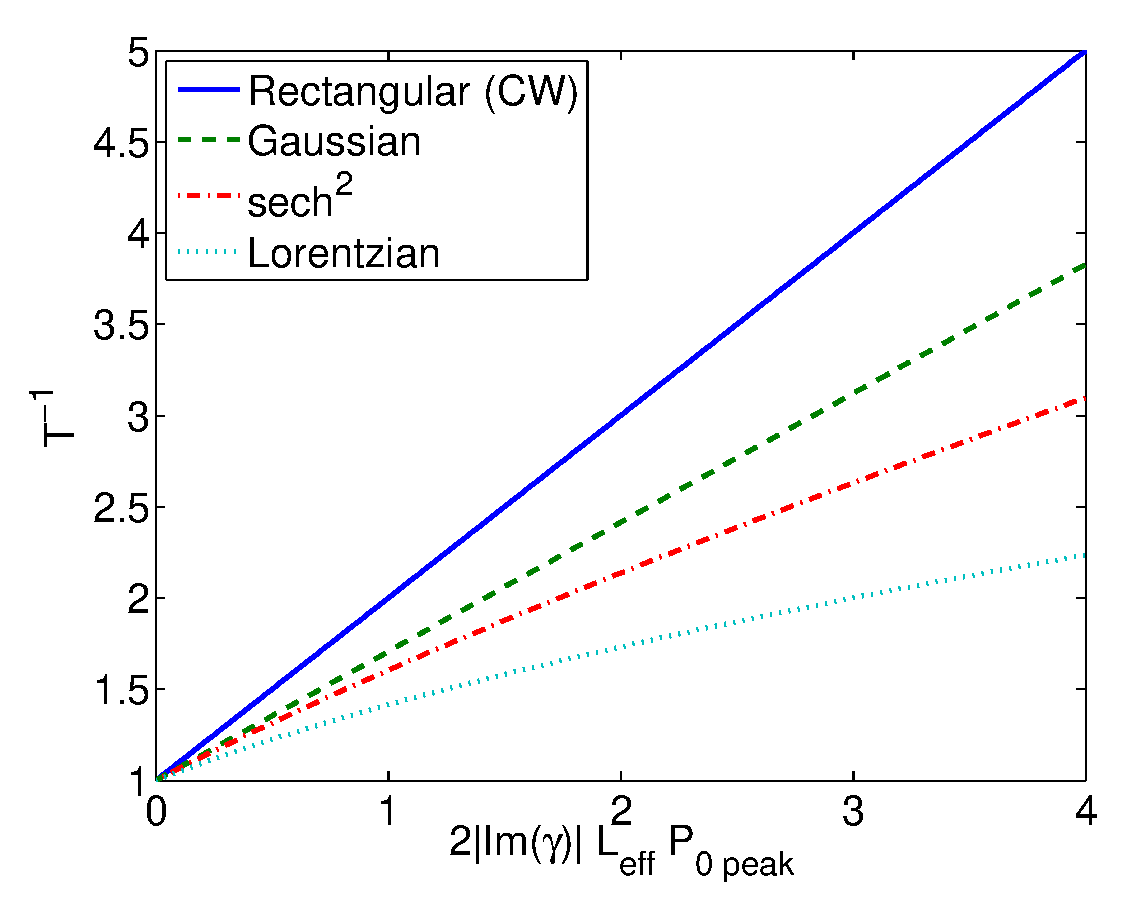
\includegraphics[width=0.5\textwidth]{imGamma_transmissionGaussianLorentzianHypSecant}
    \caption{Absorption fit to equation \ref{eq:transmissionLinear} (CW) , \ref{eq:transmissionGaussian} (Gaussian), \ref{eq:transmissionHypSecant} (Hyperbolic secant) and \ref{eq:transmissionLorentzian} (Lorentzian pulses).}
    %\caption{Absorption assuming different pulse shapes.}
    \label{fig:transmissionGaussianLorentzianHypSecant}
\end{figure}


As we can see in Figure~\ref{fig:transmissionGaussianLorentzianHypSecant}, the cw case, which is equivalent to a pulse with a rectangular shape, has a linear dependence with the peak power, while the other shapes are all sublinear, being the Lorentzian case the most sublinear. The gaussian and hyperbolic secant are quite similar.
Instead of using the exact equations shown here, some of which are a bit complicated, one can do an approximation for small $ \delta $ $(\delta \gg 1)$ to first order, where we obtain:


\begin{align}
&  \tilde{T}^{-1}_{NL~Lorentzian}   = 1 + \frac{1}{2}\delta + O(\delta^2) \\
& \tilde{T}^{-1}_{NL~Gaussian}  = 1 + \frac{2}{3}\delta + O(\delta^2) \\
& \tilde{T}^{-1}_{NL~Hyp.~secant}  = 1 + \frac{1}{\sqrt{2}}\delta + O(\delta^2)
\end{align}


remembering that $ \delta = 2|Im(\gamma)| L_{eff} P_{0 peak} $, $ \tilde{T} $ is the pulse energy transmittance, and $ \tilde{T}_{LP} $ the low-power transmittance. It is worth noting that the slopes are significantly different.

%\section{Imaginary part of Gamma coefficient}

\section{Nonlinear loss measurements: Im\{$ \gamma $\}}

We measured the nonlinear losses with a power meter using 1 picosecond laser at a wavelength of 1539~nm, and a variable attenuator. The results are shown in Fig.~\ref{fig:imGammaSamples}, where the curves were fitted to Eq.~\ref{eq:transmissionHypSecant} for $sech^2$ pulses in order to extract the nonlinear loss parameter $Im(\gamma)$ (shown in Table~\ref{table:results}).

%We measured nonlinear losses with a power meter using  1ps pulsed laser at the wavelength of 1539~nm and a variable attenuator. As the shape of the pulses was $sech^2$, we fitted $|Im(\gamma)|$ values, shown in Table~\ref{tab:results}, to equation~\ref{eq:transmissionHypSecant}.

%We measured nonlinear losses with a power meter using  1ps pulsed laser at the wavelength of 1939nm and a variable attenuator. As the shape of the pulses was $sech^2$, fit was made to equation~\ref{eq:transmissionHypSecant} and $|Im(\gamma)|$ values are in Table~\ref{tab:results}.

%We measure losses with power meters before and after the sample using a femtosecond fiber laser. Different peak pulses are obtained using a variable attenuator. Average to peak power conversion factor is 46.85dB, considering 50ns pulse repetition rate (20MHz) and 1-ps hyperbolic-secant pulses. Using an autocorrelator we measure 0.9072ps FWHM. Central wavelength is 1539nm and 2.82nm 3dB-spectral width.

%(Fig.~\ref{fig:imGammaSetup})
\begin{figure}[htb]
    \centering
    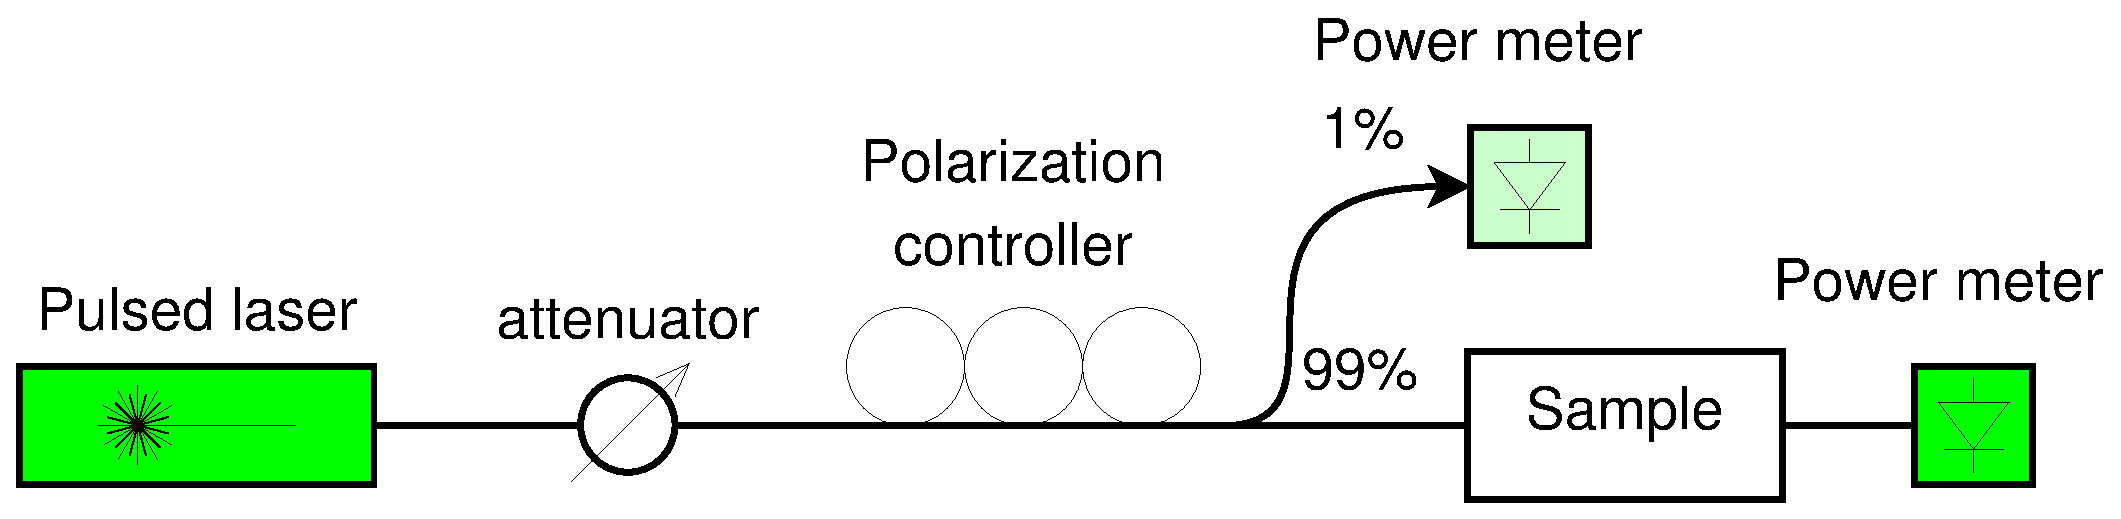
\includegraphics[width=0.80\textwidth]{imGammaFit}
    \caption{Absorption characterization setup.}
    \label{fig:imGammaSetup}
\end{figure}


\begin{figure}[htb]
    \centering
    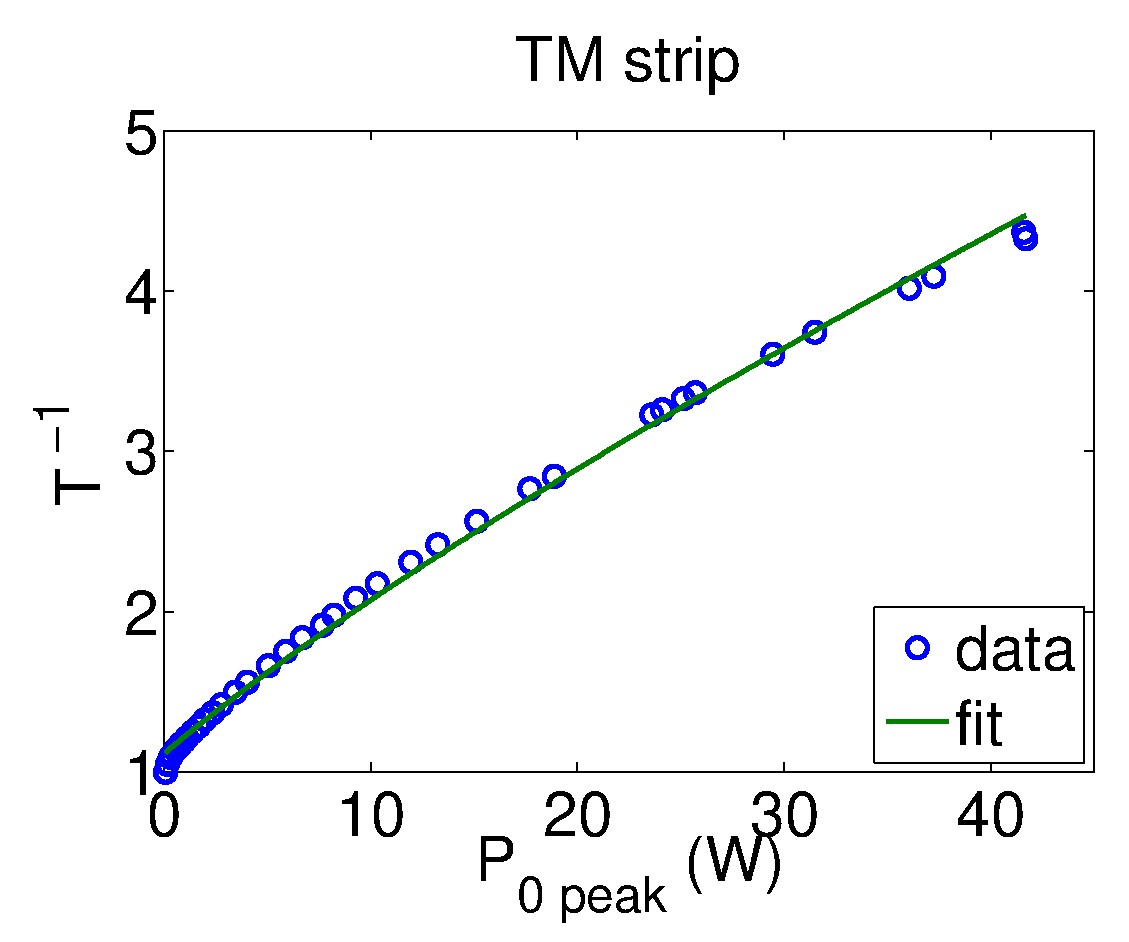
\includegraphics[width=0.39\textwidth]{imGamma_5p4366_V740TM25mm_big30}   
    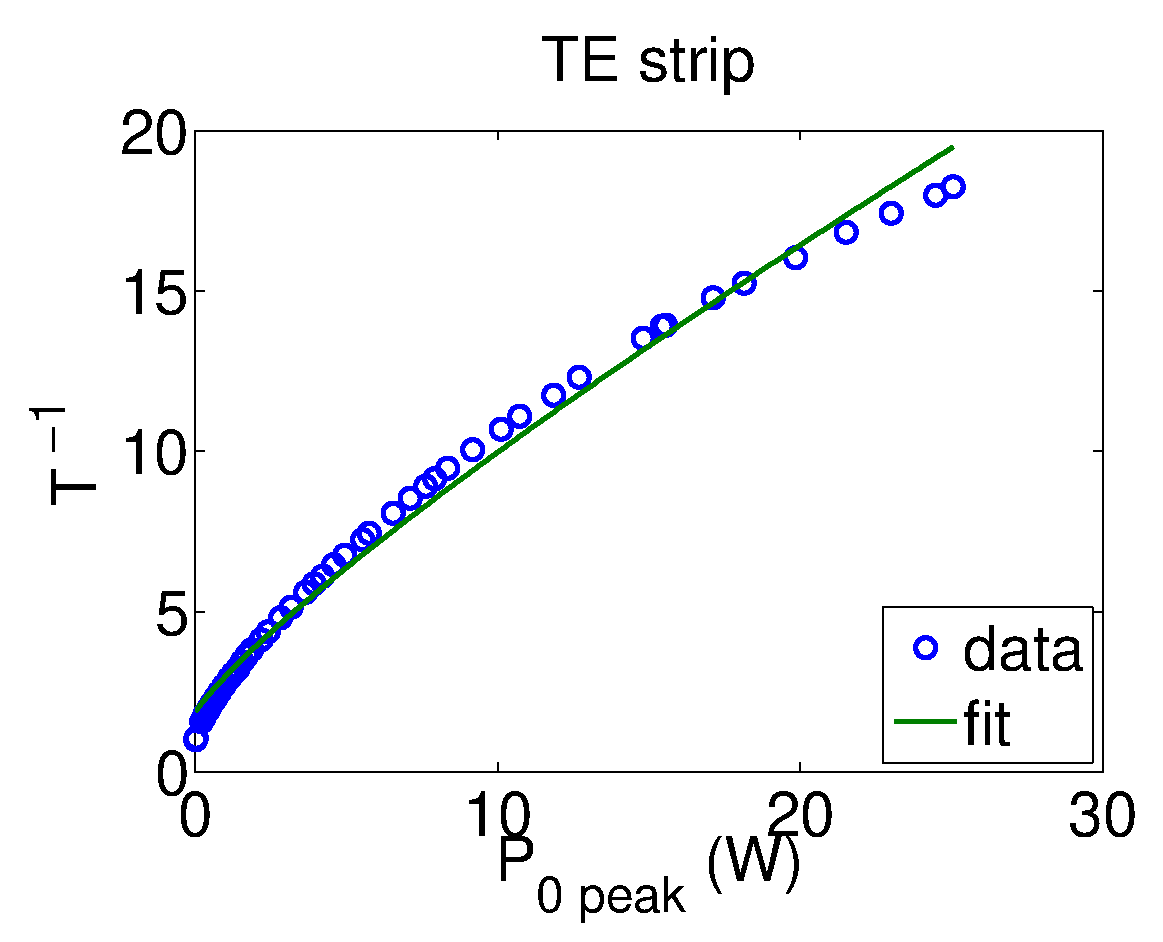
\includegraphics[width=0.40\textwidth]{imGamma_117Wm-1_V740TE25mm_big30}
    \caption{Transmission versus waveguide peak power. Fit for $ sech^2 $ pulses (Eq.~\ref{eq:transmissionHypSecant}).}
    \label{fig:imGammaSamples}
\end{figure}


\section{Results}
In Table~\ref{table:results} we see that the nonlinear absorption for TE is an order of magnitude higher than in TM waveguides. As more light travels through the Silicon, transmission reduces drastically when increasing peak power (See Figure~\ref{fig:imGammaSamples}). This is because their mode is more confined into the silicon with a higher TPA coefficient than the silica.

We have demonstrated that the linear fit is only valid for CW lasers or perfectly rectangular pulses. On the other hand, fit to equation~\ref{eq:transmissionHypSecant} matches reasonably well with the measurements  (Fig.~\ref{fig:imGammaSamples}) . Whereas commonly used equation~\ref{eq:transmissionLinear} fit underestimates $|Im(\gamma)|$ values by half (see Table~\ref{table:results}).

%The first significant result is the fact that the linear fit, only valid when using CW lasers, is a factor of two lower than the correct fit for pulsed laser. So, in order to obtain a valid fit when using averaging power meters and pulsed laser one must use equation \ref{eq:transmissionHypSecant}. Moreover in Table~\ref{tab:results} we see that the nonlinear absorption in the TE waveguide is an order of magnitude higher than in the TM waveguide, which has less power traveling through the silicon.


\begin{table}
\centering
\caption{Properties of 445x220 and 485x220nm (TE and TM) silicon strip waveguides. $|Im\{\gamma\}|$ was fitted assuming both rectangular (Eq.~\ref{eq:transmissionLinear}) and $ sech^2 $  pulses (Eq.~\ref{eq:transmissionHypSecant}).}
\begin{tabular}{l|cc}
\hline
Sample  & TM strip & TE strip\\\hline
coupling [dB] & 6 & 6\\
propagation [dB/cm]  & 1.9 & 4.9\\
Leff [mm]  & 15.2 & 8.34\\
$|Im\{\gamma\}| ~ [Wm]^{-1} $  (Eq.~\ref{eq:transmissionLinear} fit) & 2.68 & 26.71\\
$|Im\{\gamma\}| ~ [Wm]^{-1}$  (Eq.~\ref{eq:transmissionHypSecant} fit)  &  5.44 & 68.08\\
 \hline
\end{tabular}
\label{table:results}
\end{table}

%$ \frac{P_{Idler}(L)}{P_{Signal}(L)}$ for 14.46dBm pump power in waveguide gives an idea of FWM Conversion efficiency when wavelength difference between signal and pump increases. Fitting to the FWM efficiency formula in paper \cite{Vallaitis2009} we obtain -19860ps/(nm km) dispersion, 1.7dB/cm losses and $ Re\{\gamma\} = 47 (Wm)^{-1} $.}
%\section{Figure of merit}


\section{Conclusion}
In conclusion, one has to be careful when extracting the imaginary part of $ \gamma $ from pulse transmission measurements, as Eq.~\ref{eq:transmissionLinear} is only valid for instantaneous transmission values. If transmission is measured with an averaging power meter, one has to use Eq.~\ref{eq:transmissionIntegral} for the specific pulse-shape, where in this paper we provide the solution for Lorentzian, Hyperbolic secant, and Gaussian shapes.




\section*{Acknowledgments}
% We acknowledge Spanish Ministry of Science and Innovation SINADEC(TEC2008-06333) and PROMETEO/2010/087 NANOFOTONICA projects, and Universidad Polit\'ecnica de Valencia for PAID 2011/1914 and J. Matres' doctoral grant.

\end{document} 
